\documentclass[dvipdfmx]{jsarticle}
\usepackage[dvipdfmx]{graphicx}
\usepackage{url}
\title{ウツボについて}
\author{関 真成澄}
\date{\today}
\begin{document}
\maketitle
\section{はじめに}
\subsection{本レポートの目的}
本レポートでは, ウツボ（Gymnothrac kidako）の生態や特徴についてまとめ, 魅力を明らかにすることを目的とする。
\subsection{ウツボをまとめるきっかけ}
私が大阪府の海遊館という水族館を訪れた際, ウツボの正面を向いた姿が衝撃的だったからである。(図1)
\begin{figure}[htbp]
  \centering
  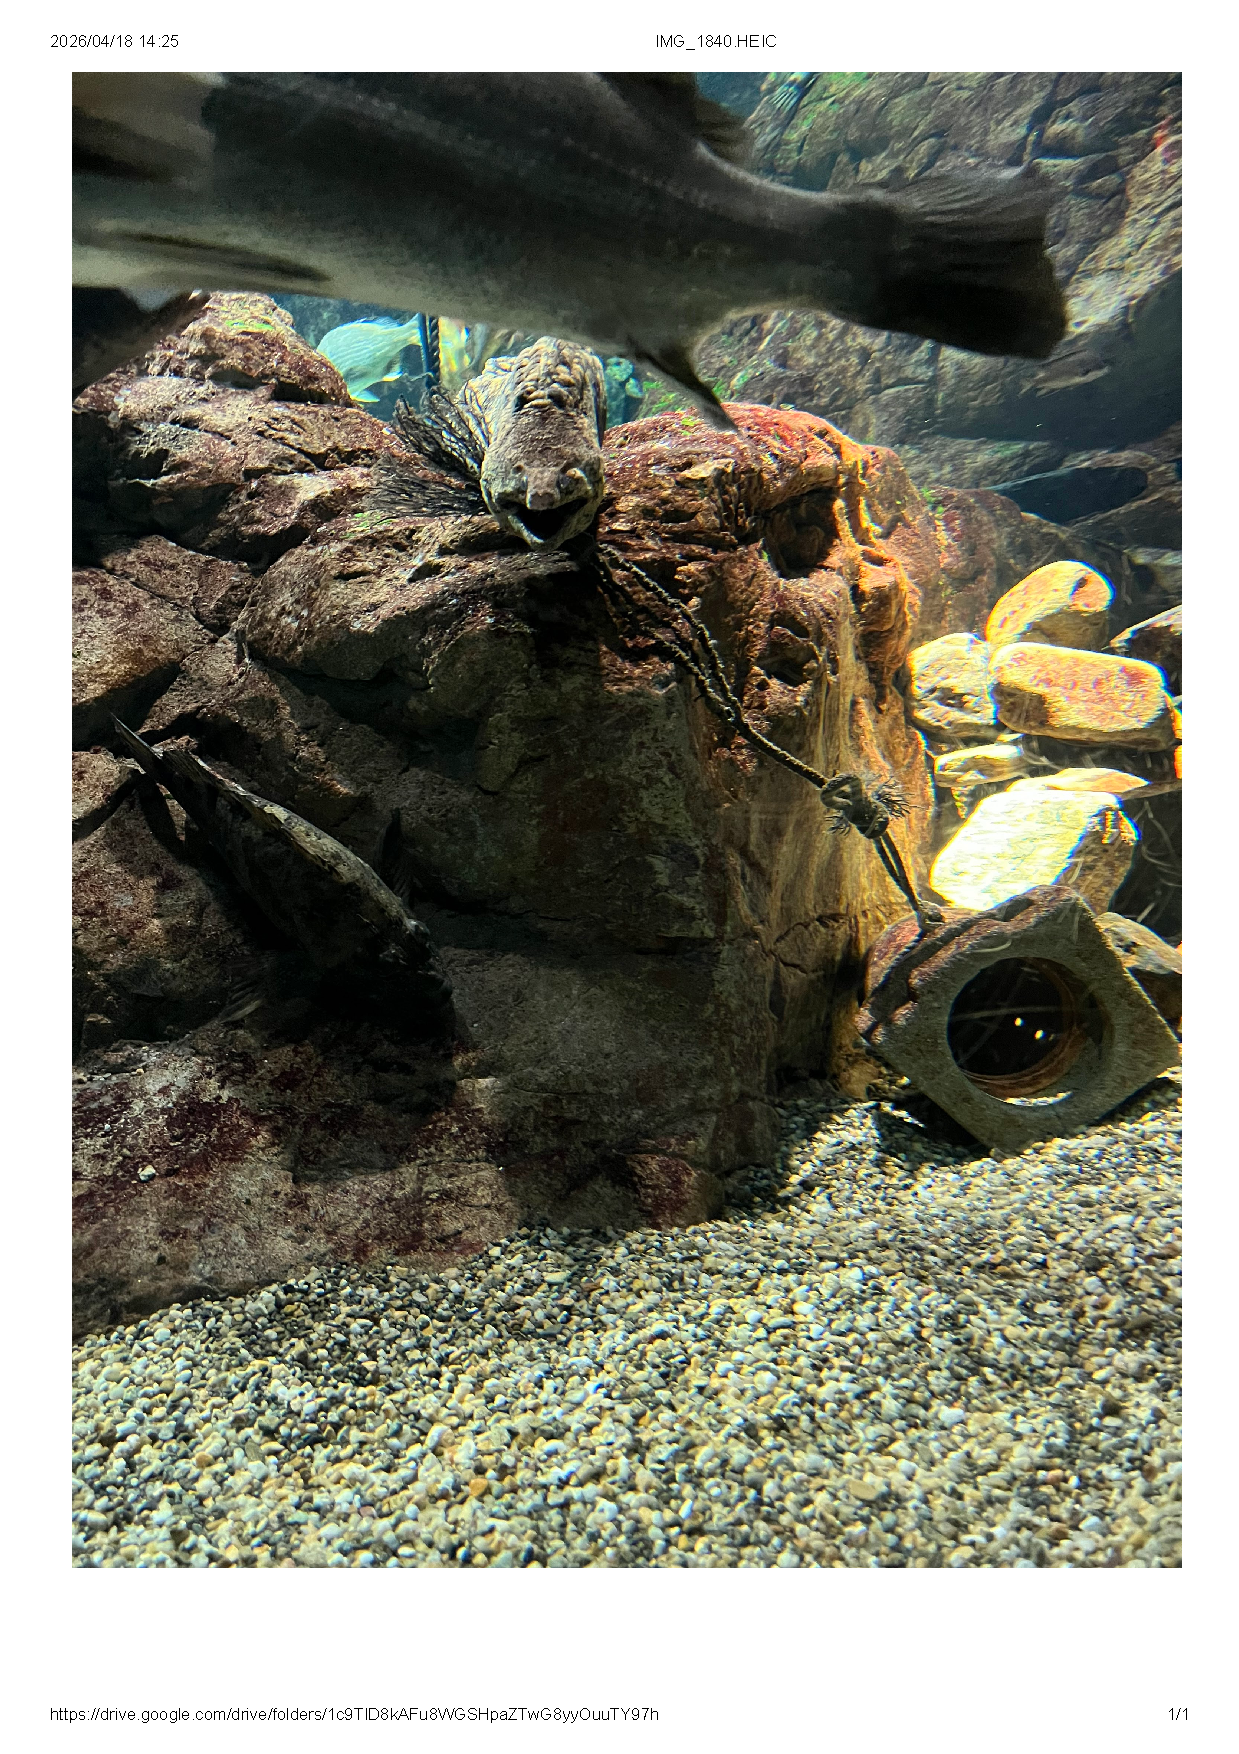
\includegraphics[width=100mm,trim=20mm 150mm 20mm 10mm, clip]{utubo1.pdf}
  \caption{ウツボの正面（2024/03/19撮影）}
  \label{fig:my_label}
\end{figure}
\section{ウツボの概要}
\subsection{分類}
ウツボはウナギ目ウツボ亜目ウツボ科の海水魚の総称である。
\subsection{生息域}
日本では島根県から九州にかけての日本海側や, 千葉県の房総半島から九州までの太平洋側などに生息している。
\subsection{名前の由来}
諸説あり, 長い矢を収める靭（うつぼ）という入れ物の形に似ているからであるという説や, 岩礁に空いた空洞（うつほら）に生息しているからという説がある。

下の図はウツボの概要を表にまとめたものである。（表1）
\begin{table}[htbp]
\centering
\begin{tabular}{|l|l|}
\hline
分類 & ウナギ目ウツボ科 \\
\hline
生息地 & 熱帯・亜熱帯の海 \\
\hline
体長 & 約30cm〜4m程度 \\
\hline
特徴 & 細長い体，鋭い歯 \\
\hline
食性 & 肉食（魚・甲殻類など） \\
\hline
\end{tabular}
\caption{ウツボの概要まとめ}
\label{tab:basic}

\raggedright
\section{面白い生態}
\subsection{共生}
クリーナーフィシュと呼ばれるホンソメワケベラやクリーナーシュリンプと呼ばれるオトヒメエビ, アカシマシラヒゲエビと共生しておりウツボは体をきれいにしてもらっている。ウツボは肉食であるが, 手あたり次第に食べてしまうのではなく, 自分の利益になるいきものとはうまく共存していることがわかる。
\subsection{性格}
見た目の通り獰猛な性格をしているイメージがあるが実際には岩の隙間に隠れて生活しており, 臆病で不用意に近づいたり, 攻撃を加えたりしなければ積極的に襲ってくることはない。



\begin{thebibliography}{9}
\bibitem{sunshine}サンシャイン水族館, 「sunshine aquarium ikiformation」\url{https://onlineshop.sunshinecity.jp/blog/post-1404/}
\end{thebibliography}
\end{table}
\end{document}
